% Created 2024-05-31 vie 17:42
% Intended LaTeX compiler: pdflatex
\documentclass[a4paper]{article}
\usepackage[utf8]{inputenc}
\usepackage[T1]{fontenc}
\usepackage{graphicx}
\usepackage{longtable}
\usepackage{wrapfig}
\usepackage{rotating}
\usepackage[normalem]{ulem}
\usepackage{amsmath}
\usepackage{amssymb}
\usepackage{capt-of}
\usepackage{hyperref}
\usepackage[spanish, american]{babel}
\usepackage{amsmath, amssymb}
\author{Adrián Arroyo Calle}
\date{Curso 2023-2024}
\title{Práctica Final - Fractales}
\hypersetup{
 pdfauthor={Adrián Arroyo Calle},
 pdftitle={Práctica Final - Fractales},
 pdfkeywords={},
 pdfsubject={},
 pdfcreator={Emacs 29.3 (Org mode 9.6.15)}, 
 pdflang={English}}
\begin{document}

\maketitle

\section{Objetivo}
\label{sec:org2e444fb}

Desarrollar una implementación paralela eficiente de un programa que genere imágenes de algún fractal usando Julia.

Se proponen diferentes tipos de fractales, cada alumno puede escoger el que prefiera. Estos fractales propuestos
son paralelizables, aunque no todos admiten las mismas técnicas. Se valorará tanto el resultado final (código) como
la presentación en la que se exponga la solución, cómo se ha llegado a ella, estadísticas para respaldar las ideas, etc

Se deberán usar tamaños de fractales (tanto de la resolución de las imágenes como de iteraciones) que permita observar
las mejoras.

\begin{center}
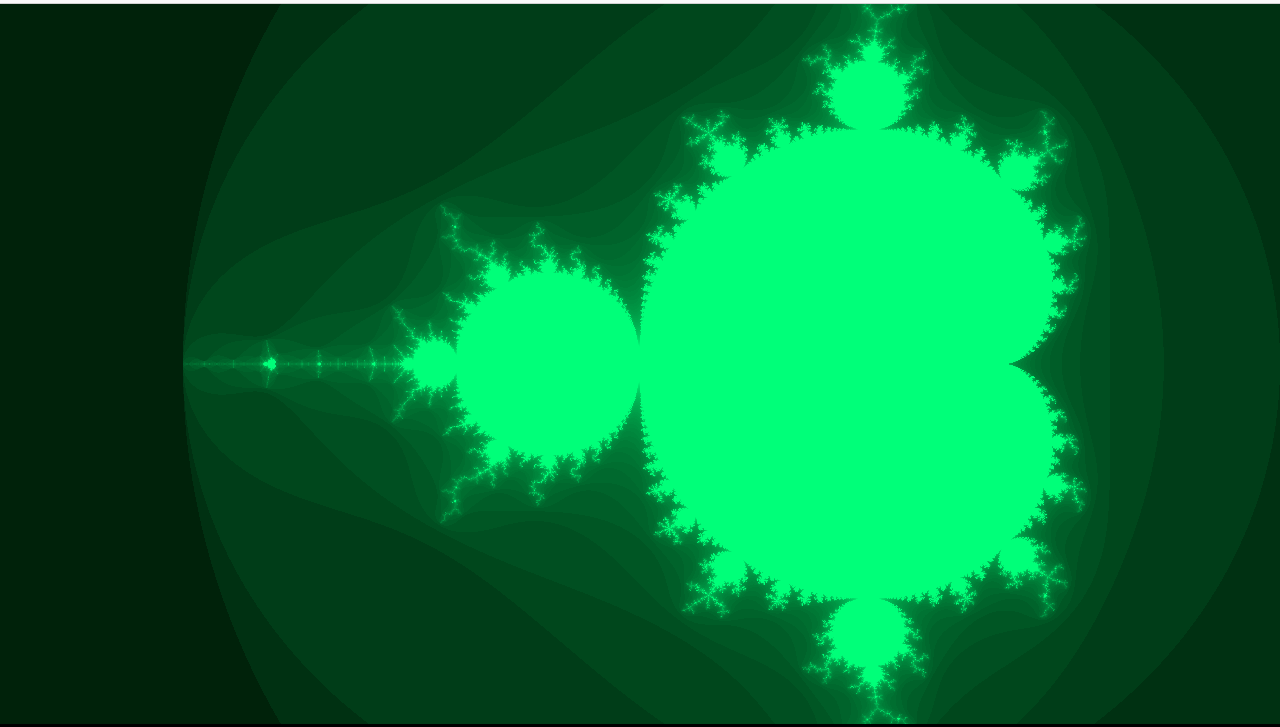
\includegraphics[width=.9\linewidth]{./Mandelbrot.png}
\end{center}

\section{Fractales}
\label{sec:org27a55cf}

Se podrá elegir uno de los siguientes fractales:

\subsection{Conjunto de Mandelbrot}
\label{sec:org7ce0e38}

Quizá el fractal más famoso. Se define sobre cada punto del plano de los números complejos (aunque por comodidad,
podemos definirlo solo entre (-2.5, 1.0) en la dimensión real y (-1, 1) en la dimensión imaginaria.

Sobre cada punto (\(c\)) se ejecuta la siguiente función recursiva:

\begin{equation}
\begin{cases}
z_0 = 0\in \mathbb{C} & \text{(termino inicial)} \qquad \\
z_{n+1} = z_n^2 + c & \text{(sucesion recursiva)}
\end{cases}
\end{equation}

Si tras N iteraciones, el valor \(z_{n}\) se se ha \emph{escapado} de una zona acotada, el punto pertenece al conjunto
de Mandelbrot. Se suele considerar que un punto \(z\) está dentro si \(\mid z \mid < 2\). A más iteraciones, más precisa
será la imagen generada del fractal.

\subsection{Conjunto de Julia}
\label{sec:orgca8ea4f}

Íntimamente relacionado con el de Mandelbrot. La fórmula de recursión es idéntica, simplemente cambia que
cada punto del plano empieza siendo \(z_{0}\) y \(c\) es una constante. Los valores de \(c\) más interesantes visualmente
son puntos cerca del borde del conjunto de Mandelbrot. El valor de escape aquí depende del fractal en concreto, aunque si nos limitamos
a \(c\) bajos (donde cada parte sea menor que 1) serán similares a los de Mandelbrot.

\subsection{Alformbra de Sierpinski}
\label{sec:org6fb5317}

Se toma una superficie cuadrada, se subdivide en 9 cuadrados y el cuadrado central se elimina. En cada uno de los 8
cuadrados restantes se realiza la misma operación. Así hasta N iteraciones.

\subsection{Helecho de Barnsley}
\label{sec:orgde39fb7}

Un fractal que tiene una gran similitud con los helechos. Utiliza números aleatorios para su construcción.

Se empieza en un punto (0,0) y se pinta, el siguiente punto en pintar es el producto de una transformación afín, que dependiendo de la probabilidad
será una u otra según probabilidades.

\begin{align}
f_1(x,y) &= \begin{bmatrix} 0.00 & 0.00 \\ 0.00 & 0.16 \end{bmatrix} \begin{bmatrix} x \\ y \end{bmatrix}
\\[6px]
f_2(x,y) &= \begin{bmatrix} 0.85 & 0.04 \\ -0.04 & 0.85 \end{bmatrix} \begin{bmatrix} x \\ y \end{bmatrix} + \begin{bmatrix} 0.00 \\ 1.60 \end{bmatrix}
\\[6px]
f_3(x,y) &= \begin{bmatrix} 0.20 & -0.26 \\ 0.23 & 0.22 \end{bmatrix} \begin{bmatrix} x \\ y \end{bmatrix} + \begin{bmatrix} 0.00 \\ 1.60 \end{bmatrix}
\\[6px]
f_4(x,y) &= \begin{bmatrix} -0.15 & 0.28 \\ 0.26 & 0.24 \end{bmatrix} \begin{bmatrix} x \\ y \end{bmatrix} + \begin{bmatrix} 0.00 \\ 0.44 \end{bmatrix}
\end{align}

La probabilidad de ejecutar \(f_{1}\) es del 1\%, \(f_{2}\) del 85\%, \(f_{3}\) del 7\% y \(f_{4}\) del 7\% restante.

\subsection{Triángulo de Sierpinski}
\label{sec:org116618c}

Existen diversas formas de generar este fractal de triángulos dentro de triángulos. Aquí se propone generarlos mediante el método
probabilístico. En este método se eligen 3 puntos como los vértices del triángulo. Se toma \(v_{n}\) aleatoriamente como un punto dentro de este triángulo.
Se toma uno de los 3 vértices. Entre la posición de \(v_{n}\) y el vértice, se toma el punto medio y se pinta. Este será \(v_{n+1}\). El proceso se repite eligiendo
aleatoriamente un nuevo vértice.

Si bien las primeras iteraciones pueden caer fuera del triángulo, eventualmente se estabilizará y todos los puntos pintados formarán parte del fractal.


\section{Paquetes recomendados}
\label{sec:orga9a0789}

Se recomienda el uso de los siguientes paquetes en el código. Los paquetes pueden instalarse de la siguiente forma:

\begin{verbatim}
julia> import Pkg
julia> Pkg.add("NombrePaquete")
\end{verbatim}

\subsection{Images}
\label{sec:org11983d6}

Para generar el resultado como una imagen. Images trae una función \texttt{save} que toma un fichero de salida y una matriz de píxeles. Soporta los formatos más comunes como PNG.

\begin{verbatim}
using Images

a = fill(RGB{Float64}(1.0, 0.0, 0.0), (100, 100)) # matriz 100x100 de color rojo
save("imagen.png", a)
\end{verbatim}

\subsection{ColorSchemes}
\label{sec:org09d2142}

Mapas de colores. Para un número 0 y 1, devuelven un color. Útil para ciertos fractales. Los colores son compatibles con Images.

\begin{verbatim}
using ColorSchemes

julia> using ColorSchemes

get(colorschemes[:delta], 0.0)
# RGB{Float64}(0.0659773860137986,0.12386004993819841,0.24948115997128678)

get(colorschemes[:delta], 1.0)
# RGB{Float64}(0.09053276383981979,0.13733860758438335,0.07325761429945674)
\end{verbatim}

\section{Exposición}
\label{sec:org2da641d}

Se valorará la exposición del trabajo frente a la clase. Se dará un tiempo de 10 minutos para presentar el trabajo. Se admitirán preguntas al finalizar la exposición.

\section{Entrega}
\label{sec:org7ebe085}

Se entregará el código y un fichero de instrucciones para ejecutarse en el Campus Virtual en el apartado habilitado para tal efecto.
\end{document}
